\documentclass{article}
\usepackage{graphicx,float}
\usepackage{listings}
\usepackage{xcolor}
\usepackage{amsmath}
\usepackage{geometry}
\geometry{left=2.0cm,right=2.0cm,top=2.5cm,bottom=2.5cm}

\lstset{numbers=left,
numberstyle=\tiny,
keywordstyle=\color{blue}, commentstyle=\color[cmyk]{1,0,1,0},
frame=null,
%rulesepcolor=\color{red!20!green!20!blue!20},
basicstyle=\ttfamily\small,
xleftmargin=2em,
xrightmargin=2em,
aboveskip=1em,
showspaces=false
}

\author{Yifan Zhao}
\title{Automatical Learning and Data Mining\\HW3 Report}
\begin{document}
 \maketitle
 \section{Descriptions}
 \subsection{}The data set contains 36000 cases in total.
 \subsection{}This data set contains temporal data from three sensors worn by an actor performing 5 kinds of activities: bending(two different ways), cycling, lying down, sitting, standing, walking. So the classification task is to recognize these activities by the data of the sensors.
 \subsection{}There are 6 descriptors. All of them are continuous real numbers. Descriptor 1,3 and 5 are the mean value of sensors 1,2 and 3, and descriptor 2,4 and 6 are the variances, respectively.
 \subsection{}Each class is a kind of activity. The classes cycling, lying down, sitting, standing, walking have the same number of cases 7200.
 \section{Architecture}
 \subsection{}For the classes cycling, lying down, sitting, standing, walking, there are 1920 cases in the test set, the rest in the training set. The proportions of cases in each class for the test set and the training set are exactly the same, $\frac{1}{5}$.
 \subsection{}Since the value of each descriptor is a real number, we could directly set it as the component of the input vector. Once we have the input, we could compute the value of each node in the hidden layer. For any integer i in [1,h], the value of the node \[y_{i}=f(\sum\limits^{p_{0}}_{j=1}w_{ij}x_{j}+b_{i})\]
 For the true output prescribed for each input in the database, we store it with each input as a 5-dimension vector whose components are all 0 or 1(1 for the class it belongs to, 0 for otherwise).
 Then for the output layer, we have a similar formula to the input: for any integer k in $[1,p_{2}]$, the value of the node
 \[z_{k}=f(\sum\limits^{h}_{i=1}w_{ki}y_{i}+b_{k})\]
 Then we have the output vector.
 We can apply the softmax function to the output vector to transform its length to 1. Then the output vector could be a probability distribution of the case's class. To decide into any class, we compute its argmax i.e., the greatest component's index, the result will be a integer in [1,5], this integer is its class index according to the MLP.\\
 Then we compute the cross entropy or the squared norm between this probability vector and the correct output. The cross entropy between correct output vector $Z=(z_{1},\dots,z_{p_{2}})$ and the output vector by MLP $\hat{Z}=(\hat{z}_{1},\dots,\hat{z}_{p_{2}})$ is defined by
 \[CE(Z,\hat{Z})=\sum\limits^{p_{2}}_{i=1}z_{i}log\frac{z_{i}}{\hat{z}_{i}}\]
 Relevant Python codes are as follows:
 \begin{lstlisting}[language=Python]
#import the data set
trains = [[], [], [], [], []]
tests= [[], [], [], [], []]
for k in range(1, 6):
    #the training set
    for i in range(1, 12):
        df = pd.read_csv('F:/Files/DataMining/HW2/' + str(k) + '/dataset' + str(i) + '.csv',
                         usecols=[1, 2, 3, 4, 5, 6],skiprows=[0, 1, 2, 3, 4], header=None)
        #insert the correct output behind each case
        for j in range(6, 11):
            if j == k + 5:
                df.insert(loc=j, column=str(j + 1), value=np.ones([len(df), 1]))
            else:
                df.insert(loc=j, column=str(j + 1), value=np.zeros([len(df), 1]))
        trains[k-1].extend(df.values)
    #the test set
    for i in range(12,16):
        df = pd.read_csv('F:/Files/DataMining/HW2/' + str(k) + '/dataset' + str(i) + '.csv',
                         usecols=[1, 2, 3, 4, 5, 6],skiprows=[0, 1, 2, 3, 4], header=None)
        for j in range(6, 11):
            if j == k + 5:
                df.insert(loc=j, column=str(j + 1), value=np.ones([len(df), 1]))
            else:
                df.insert(loc=j, column=str(j + 1), value=np.zeros([len(df), 1]))
        tests[k-1].extend(df.values)
 \end{lstlisting}
\section{Size of The Hidden Layer}
We use the Python package matplotlib to do PCA in Python. The eigenvalues are stored in the component fracs of the result. Because this data set has only 6 descriptors but 36000 cases, so the reduction of dimension by PCA is not effective. To preserve 95\% of the total sum of eigenvalues, we need all 6 eigenvalues. Similar situation for the PCA of each class separately. Thus we have the small size s=6, the intermediate size S=26, a larger size SL=52.\\
Relevant Python codes are as follows:
\begin{lstlisting}[language=Python]
#use PCA to decide the size of the hidden layer
d1 = []
d = [[], [], [], [], []]
pca1 = []
pca = [[], [], [], [], []]
count1 = 0
count = np.zeros(5)
for k in range(1, 6):
    for i in range(1, 16):
        df = pd.read_csv('F:/Files/DataMining/HW2/' + str(k) + '/dataset' + str(i) + '.csv',
                         usecols=[1, 2, 3, 4, 5, 6],skiprows=[0, 1, 2, 3, 4], header=None)
        d[k - 1].extend(df.values)
    d[k - 1] = np.asarray(d[k - 1])
    pca[k - 1] = PCA(d[k - 1])  #do PCA for each class
    d1.extend(d[k - 1])
    #compute the number of eigenvalues preserving 95% of the total sum of eigenvalues
    for m in range(6):
        count[k - 1] += pca[k - 1].fracs[m]
        if count[k - 1] >= 0.9:
            break
    count[k - 1] = m + 1
d1 = np.asarray(d1)
pca1 = PCA(d1)  #do PCA for the whole data set
for m in range(6):
    count1 += pca1.fracs[m]
    if count1 >= 0.95:
        break
#compute the size of the hidden layer
s = m + 1
S = sum(count)
SL = 2 * S
\end{lstlisting}
\section{Inplementing of Learning}
We choose to use tensorflow and its API in Python.
\subsection{}We choose MSE as our loss function. Tensorflow has a very convenient MSE function: tf.losses.mean\_squared\_error. The training set has 26400 cases, the test set has 9600 cases. The frequencies of each class in the both sets are equal, $\frac{1}{5}$.
\subsection{}With tensorflow, we could generate normal distributed tensors for initialization of the wights. \\
For batch learning, we use the function np.random.choice in Python package numpy to obtain a batch. This function returns a random sample from the population with a given size.\\
For the successive gradient descent steps sizes, we assign a learning rate variable valued $\frac{\epsilon}{n}$to control the step size of gradient, where n the current number of global learning steps.\\
The stopping criterion of learning is when the norm of gradient is smaller than a given level: e.g., 0.03.
For intermediary outputs to monitor learning quality, we compute and print the prediction accuracy per 60 batches. The prediction accuracy is defined by the percentage of the correct predictions out of the whole batch.\\
Relevant Python codes are as follows:
\begin{lstlisting}[language=Python]
#compute the hidden layer
fc1 = fc_layer(x, h, 'Hidden_layer', use_relu=True)
#compute the output layer
output_logits = fc_layer(fc1[0], n_classes, 'Output_layer', use_relu=False)

#define the loss when we use MSE
with tf.name_scope('RMSE'):
    loss = tf.sqrt(tf.losses.mean_squared_error(labels=y,
     predictions=tf.nn.softmax(output_logits),name='RMSE'))
    tf.summary.scalar('RMSE',loss)
#define the loss when we use cross entropy
loss = tf.reduce_mean(tf.nn.softmax_cross_entropy_with_logits_v2(labels=y,
                     logits=output_logits[0]), name='RMSE')

#since ADAM optimizer is also a kind of gradient descent algorithm,
#we could define the optimizer as follows
with tf.name_scope('Optimizer'):
    optimizer = tf.train.AdamOptimizer(learning_rate=learning_rate,
                                         name='Op').minimize(loss)

#the weight initialization function
def weight_variable(name, shape):
    #generate the normal distributed initialized weights
    initer = tf.truncated_normal_initializer(stddev=0.01)
    return tf.get_variable('W_' + name,
                           dtype=tf.float64,
                           shape=shape,
                           initializer=initer)

#the batch function
def batch(batch_size, dataset):
    #generate the random sample
    index=np.random.choice(a=len(dataset),size=batch_size,replace=False)
    results=dataset[index,:]
    features=results[:,0:6]
    labels=results[:,6:11]
    rest=np.setdiff1d(np.arange(len(dataset)), index)
    return features,labels,rest

#compute the number of correct predictions
correct_prediction = tf.equal(tf.argmax(output_logits[0], 1), tf.argmax(y, 1), name='co_pre')
#compute the percentage of correct predictions out of the whole batch
accuracy = tf.reduce_mean(tf.cast(correct_prediction, tf.float64), name='accuracy')

#the stopping criterion
if grad_batch<0.03:
    break
    break #break the epoch and stop the learning
\end{lstlisting}
\subsection{The Curves of RMSE, $||\Delta W||$, G}
The RMSE has been computed in the loss function. We need to compute the $||\Delta W||$ and G during the learning.
\begin{lstlisting}[language=Python]
#compute the norm of the difference between the weights of the former and the present batches
delta_W=tf.square(tf.norm(fc1[1]-W_in2hid_form))+
        tf.square(tf.norm(output_logits[1]-W_hid2out_form))
delta_b=tf.square(tf.norm(fc1[2]-b_in2hid_form))+
        tf.square(tf.norm(output_logits[2]-b_hid2out_form))
with tf.name_scope('Delta_Wb'):
    difference=tf.sqrt(delta_W+delta_b,name='Delta_Wb')
    #plot the curve
    tf.summary.scalar('Delta_Wb',difference)
#compute the gradient
with tf.name_scope('Gradient'):
    gradient=tf.multiply(learning_rate,difference,name='Gradient')
    #plot the curve
    tf.summary.scalar('Gradient', gradient)
\end{lstlisting}
As the codes have shown, we first compute the norm of the difference of weights and biases separately. Then we add the squared norms together. In this way we could avoid to manipulate the matrices of weights and biases, which are pretty complicated. The computation of gradient is easy after we have the weights' difference, just multiply it with the learning rate.\\
Then we could plot the curves with the visualization toolkit tensorboard.
  \begin{figure}[H]
  \centering
  % Requires \usepackage{graphicx}
  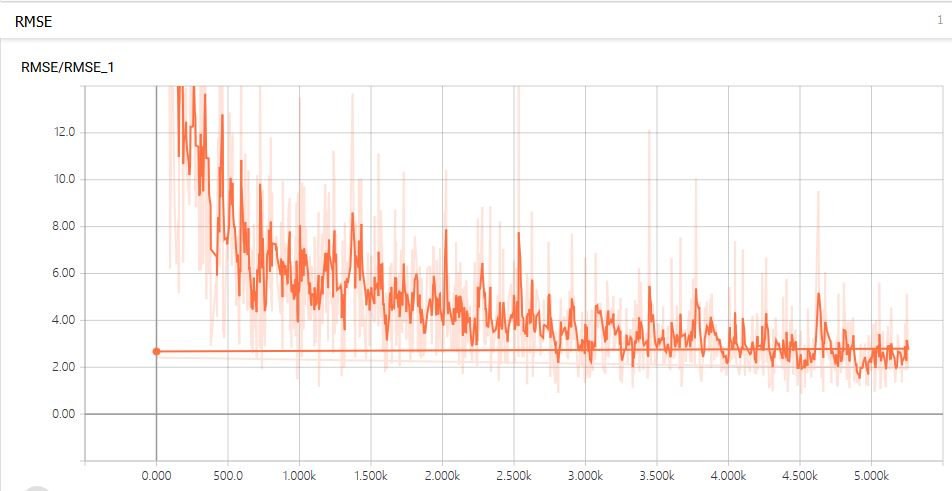
\includegraphics[width=0.75\textwidth]{RMSE.jpg}
  \caption{RMSE}\label{}
  \end{figure}
  \begin{figure}[H]
  \centering
  % Requires \usepackage{graphicx}
  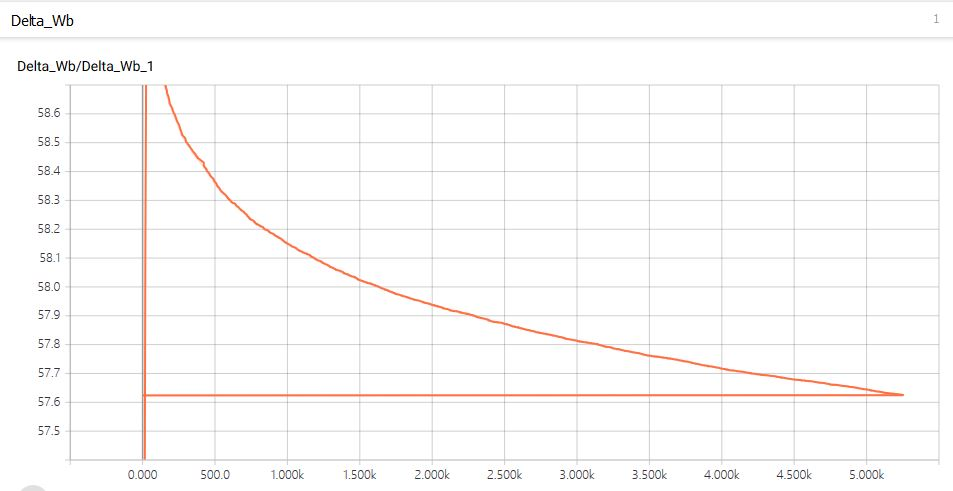
\includegraphics[width=0.75\textwidth]{DeltaWb.jpg}
  \caption{$||\Delta W||$}\label{}
  \end{figure}
  \begin{figure}[H]
  \centering
  % Requires \usepackage{graphicx}
  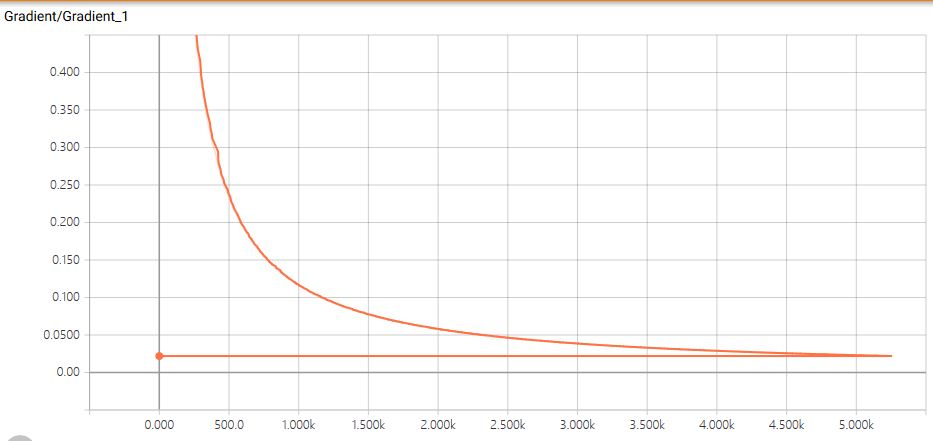
\includegraphics[width=0.75\textwidth]{Gradient.jpg}
  \caption{G}\label{}
  \end{figure}
As we could see,all three curves decline in an exponential shape as the global steps grow. The fluctuation of RMSE is the greatest among these three curves. The declination of $||\Delta W||$ is relatively insignificant comparing with the other two. Therefore, the declination of gradient actually is also insignificant since the shape of its curve is almost the shape of function \[f(x)=\frac{constant}{n}\]The MLP should be improved for this.
\section{Evaluation of Terminal MLP}
\subsection{}The RMSE on the whole training set is 0.73, the RMSE on the whole test set is 0.97. Although the test set has a greater RMSE, but these two values are in the same order of magnitude. So we could consider that the MLP is not over-parametrized.\\
We compute the absolute values of coordinates of the gradient by the following codes:
\begin{lstlisting}[language=Python]
#compute the absolute values of the coordinates of the gradient and plot the histograms
with tf.name_scope('Grads_W_in2hid'):
    grads_W_in2hid=tf.stack(tf.abs(tf.gradients(loss, fc1[1],stop_gradients=fc1[1],
                                                name='Grads_W_in2hid')))
    tf.summary.histogram('Grads_W_in2hid',grads_W_in2hid)

with tf.name_scope('Grads_W_hid2out'):
    grads_W_hid2out=tf.stack(tf.abs(tf.gradients(loss,output_logits[1],
                                    stop_gradients=output_logits[1],name='Grads_W_hid2out')))
    tf.summary.histogram('Grads_W_hid2out',grads_W_hid2out)
\end{lstlisting}
The computation is simple in tensorflow with the function tf.gradients.\\
We plot two histograms for the gradients for the weights of two layers separately:
  \begin{figure}[H]
  \centering
  % Requires \usepackage{graphicx}
  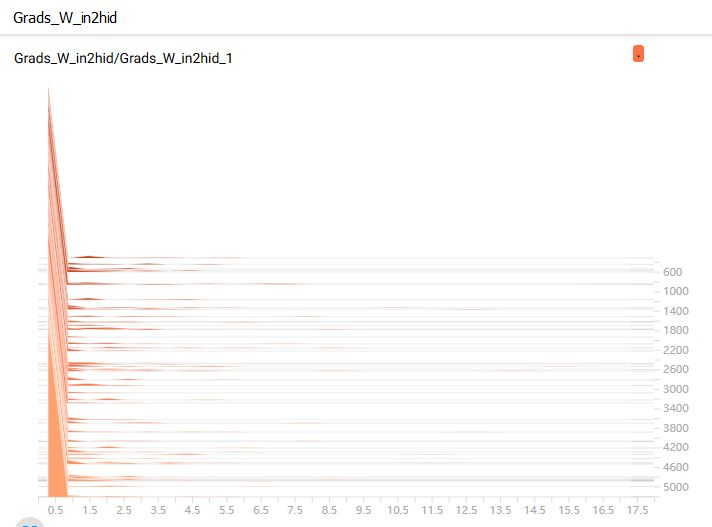
\includegraphics[width=0.75\textwidth]{G_W_in2hid.jpg}
  \caption{Gradient of weights between input and hidden layer}\label{}
  \end{figure}
  \begin{figure}[H]
  \centering
  % Requires \usepackage{graphicx}
  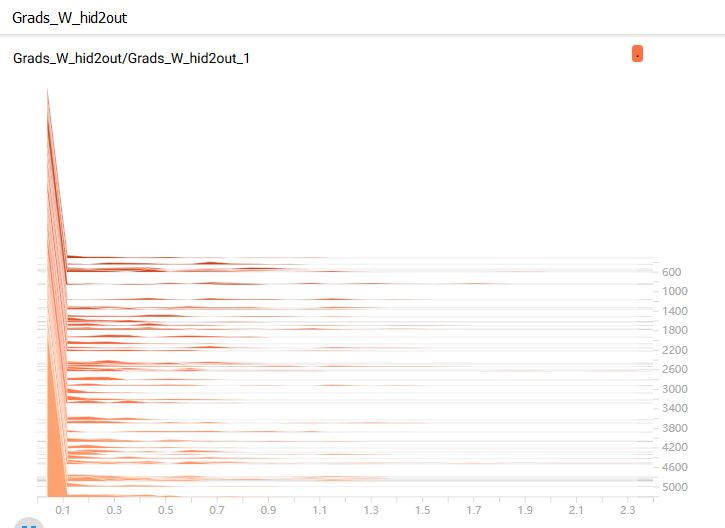
\includegraphics[width=0.75\textwidth]{G_W_hid2out.jpg}
  \caption{Gradient of weights between hidden and output layer}\label{}
  \end{figure}
According to the histograms, the number of coordinates that are exactly or roughly zero are huge and overwhelming. Thus we could consider that the gradient is zero.
\subsection{The Confusion Matrices}
\begin{lstlisting}[language=Python]
#the variable that signifies the class of denominator
indice=tf.placeholder(tf.int64,shape=[1],name='Index')
#initialization of the two matrices
entry_train=[[], [], [], [], []]
entry_test=[[], [], [], [], []]
#compare the output vector to the given class index
#and count the numbers in order to compute the numerator
prediction = tf.equal(tf.argmax(output_logits[0], 1), indice)
#compute the ratio of prediction and the number of cases in one class
ratio = tf.reduce_mean(tf.cast(prediction, tf.float64))

for i in range(5):
    label[i] = y_train[:, i] == 1
    label_test[i] = y_test[:, i] == 1
    #run the tensor ratio and store the results to a matrix
    for j in range(5):
    entry_train[i].append(sess.run(ratio,
                        feed_dict={x:x_train[label[i]],indice:[j]}))
    entry_test[i].append(sess.run(ratio,
                        feed_dict={x: x_test[label_test[i]],indice:[j]}))
\end{lstlisting}
As the codes have shown, we first assign a variable that signifies the class that the cases truly belonged to. Then we compare the class predicted by the output vector with this index variable. Then we compute the ratio of each kind of prediction. Finally after running the session, we could store the results to two matrices and output them.\\
The training confusion matrix:\\
$[0.7238636363636364,\ 0.003977272727272727,\ 0.006439393939393939\ 0.0,\ 0.265719696969697]$\\
$[0.000946969696969697,\ 0.8005681818181818,\ 0.08958333333333333,\ 0.08844696969696969,\ 0.020454545454545454]$\\ $[0.0028414472437961733,\ 0.37715476415987875,\ 0.4995264254593673,\ 0.07501420723621897,\ 0.04546315590073877]$\\ $[0.005871212121212121,\ 0.11022727272727273,\ 0.014772727272727272,\ 0.8615530303030303,\ 0.007575757575757576]$\\ $[0.34337121212121213,\ 0.015151515151515152,\ 0.058712121212121215,\ 0.0001893939393939394,\ 0.5825757575757575]$\\
The test confusion matrix:\\
$[0.7328125,\ 0.005729166666666666,\ 0.004166666666666667,\ 0.0, 0.25729166666666664]$\\
$[0.0005208333333333333,\ 0.6572916666666667,\ 0.17447916666666666,\ 0.16145833333333334,\ 0.00625]$\\
$[0.0010416666666666667,\ 0.42239583333333336,\ 0.26666666666666666,\ 0.2864583333333333,\ 0.0234375]$\\ $[0.0067708333333333336,\ 0.2140625,\ 0.022916666666666665,\ 0.7473958333333334,\ 0.008854166666666666]$\\ $[0.39791666666666664,\ 0.034895833333333334,\ 0.027604166666666666,\ 0.0010416666666666667,\ 0.5385416666666667]$\\
According to the confusion matrices, every class the training set has similar accuracy to the test set. And we could see that the accuracy of the third class is the lowest, the accuracy of the second class is the highest.
\section{Impact of Various Learning Options}
When the batch size is small, the memory could be saved a lot but the velocity of convergence will be lower. When the batch size is relatively large, the training needs a larger memory than the small batches, although the convergence might be quick. Therefore, we need an appropriate batch size.\\
For the initialization, since our initial weights are normal distributed variables with standard deviation=0.01, the relationship between the learning quality and initialization is still unclear. But I think more training epochs could compensate it even if the initial weights are not good enough.\\
Considering the velocity of convergence, an excessively small gradient descent step size sequence is not sufficient for the learning to convergent. However, large gradient descent step size sequence also has some disadvantages. As the number of global step grows, a large gradient descent step size could cause the learning accuracy to fluctuate among several fixed levels instead of converging to a limit. Thus gradient descent step size should be moderate.\\
As for this data set, the learning quality of the hidden layer size SL is the best among three different sizes. The reason may be that this data set has a small number of descriptors. And the hidden layer size SL=52 is still not a very great number. If the dimension is much greater, then the learning quality may descend.\\
\section{PCA of Hidden Layer}
Since we only have 6 descriptors for the original data, when the dimension of hidden layer is greater than 6, the hidden vectors will be rough multi-colinearity even if we have nonlinear response function. So the plot and scatter we show are only those for dimension of hidden layer=s=6 since the PCA for S and SL are meaningless.
  \begin{figure}[H]
  \centering
  % Requires \usepackage{graphicx}
  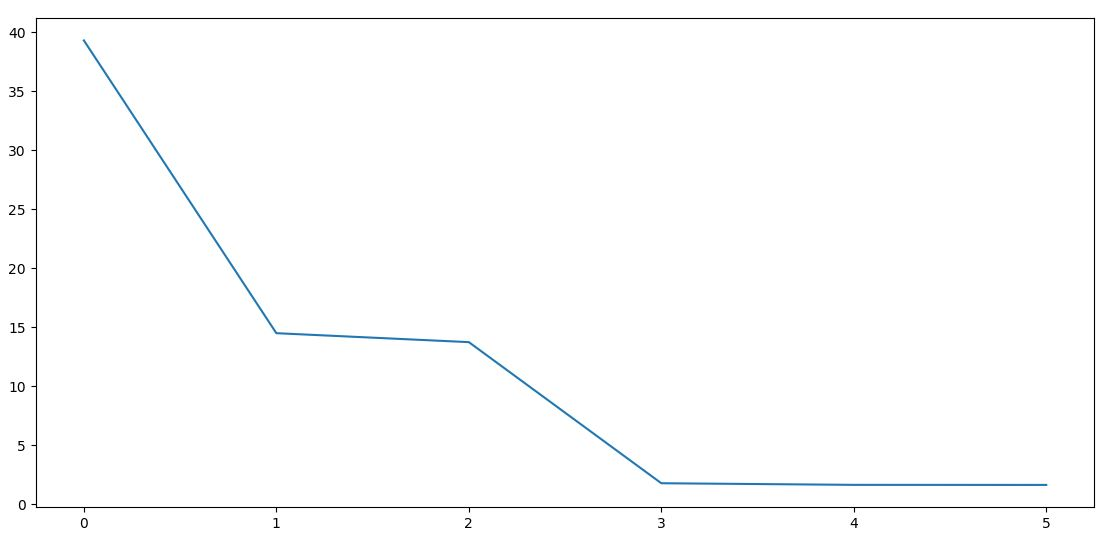
\includegraphics[width=0.75\textwidth]{Eig.jpg}
  \caption{Eigenvalues in descending order}\label{}
  \end{figure}
  \begin{figure}[H]
  \centering
  % Requires \usepackage{graphicx}
  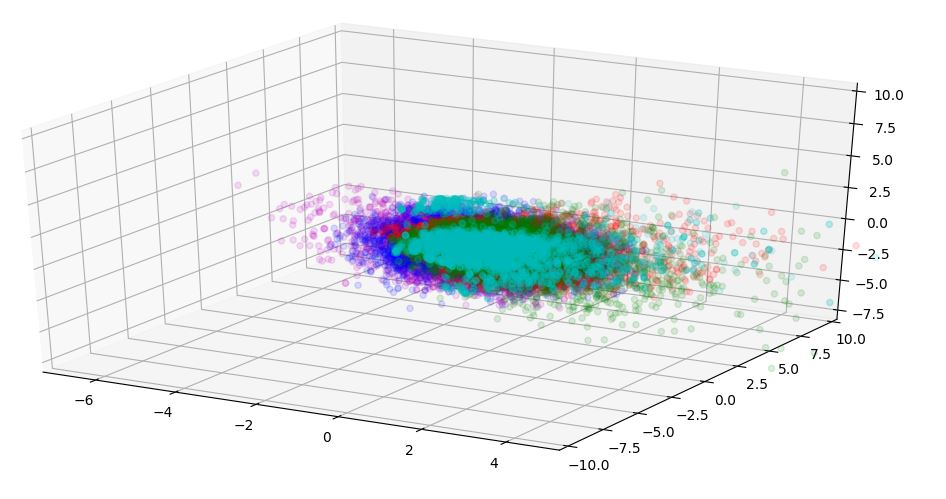
\includegraphics[width=0.75\textwidth]{Scatter.jpg}
  \caption{Points of the Projections on the First Three Eigenvectors}\label{}
  \end{figure}
As we can see from the graph, the points of the same class are clustered while points of different classes are separate. It shows that the PCA of hidden layer vectors is more effective than that of the input vectors.\\
The relevant Python codes are as follows:
\begin{lstlisting}[language=Python]
    #extract the terminal hidden layer vectors
    label = [[], [], [], [], []]
    hidden = sess.run(fc1, feed_dict=feed_dict_train)[0]
    hidden_pca = PCA(hidden) #do the PCA
    color = ['b', 'g', 'r', 'c', 'm']# initialize colors for different classes
    fig = plt.figure()
    ax = fig.add_subplot(111, projection='3d')
    for i in range(5):
        label[i] = y[:, i] == 1 #extract the index for each class
        ax.scatter(hid_pca.Y[label[i],0],hid_pca.Y[label[i],1],
                    hid_pca.Y[label[i],2],c=color[i]) #plot the points
    plt.plot(np.arange(len(pca1.mu)),pca1.mu) #plot the eigenvalues
    plt.show()
\end{lstlisting}
Since the whole script is too long, the .py files will be attached in my email. HW3.py is the main executive file and ops.py is the associated functions.
\end{document}
